\documentclass[10pt]{article}
\usepackage[usenames]{color} %used for font color
\usepackage{amssymb} %maths
\usepackage{amsmath} %maths
\usepackage{url} %maths
\usepackage[utf8]{inputenc} %useful to type directly diacritic characters
\usepackage{fancyhdr}
% customize fancyhdr package
\pagestyle{fancy} \fancyhf{}
\lhead{
\includegraphics[width=1.5cm]{uni-logo.png}
 \hspace*{.2ex}\parbox[b]{.85\textwidth}{\footnotesize
\hfill   Exercises Week 46 in DM561, 2021, IMADA, SDU}}
\rfoot{Page \thepage}

\usepackage{tikz}
\usetikzlibrary{graphs,graphdrawing}
\usegdlibrary{trees, force}

\begin{document}

\noindent {\bf Exercise 1:}\\
Let $P_1$ and $P_2$ be two permutation matrices. Is $P_1 \times P_2$ also a permutation matrix? Argue for or against your answer.\\

\noindent {\bf Exercise 2:}\\
\begin{enumerate}
\item Draw the graphs $G_A$ and $G_B$ for which the following 2 adjacency matrices $A$ and $B$ are given.
\begin{equation*}
A= \left(\begin{array}{ccccc}
           0 & 1 & 1 & 1  \\
           1 & 0 & 1 & 0  \\
           1 & 1 & 0 & 1  \\
           1 & 0 & 1 & 0  
\end{array}\right)
B= \left(\begin{array}{ccccc}
           0 & 1 & 1 & 0  \\
           1 & 0 & 1 & 1  \\
           1 & 1 & 0 & 1  \\
           0 & 1 & 1 & 0  
\end{array}\right)\hspace{1cm}
\end{equation*}
\item Are the two graphs isomorphic?
\item How many different representations (in terms of adjacency matrices) of $G_A$ are there?
\item How many different representations (in terms of adjacency matrices) of $G_B$ are there?
\item Is there a permutation matrix $P$ such that $A=P\left(PB\right)^T$ holds? 
\item If so, give all matrices $P$, such that  $A=P\left(PB\right)^T$ holds.
\end{enumerate}

\noindent {\bf Exercise 3:}\\[1cm]
Given the following graph:\\

 \begin{tikzpicture}[spring layout]    
\tikz [spring electrical layout, node distance=1.3cm,
every edge/.style={
decoration={coil, aspect=-.5, post length=1mm,
segment length=1mm, pre length=2mm},
decorate, draw}]
{
\foreach \i in {1,...,3}
\node (node \i) [fill=blue!30, text=blue!30, circle] {\i};
\draw 
(node 1) edge (node 2) edge (node 3) 
(node 2) edge (node 1) edge (node 3);
}
\end{tikzpicture}
\begin{enumerate}
\item Give an adjacency matrix $A$ for the graph. (How many different are there?)
\item For your chosen adjacency matrix, how many permutation matrices $P$ are there, such that
  $A=P\left(PA\right)^T$ holds? (Remark: this number corresponds to the size of the so-called ``automorphism group'' of the graph). 
\end{enumerate}
\newpage

\noindent {\bf Exercise 4:}\\[1cm]
Given the following graph:\\

 \begin{tikzpicture}[spring layout]    
\tikz [spring electrical layout, node distance=1.3cm,
every edge/.style={
decoration={coil, aspect=-.5, post length=1mm,
segment length=1mm, pre length=2mm},
decorate, draw}]
{
\foreach \i in {1,...,5}
\node (node \i) [fill=blue!30, text=blue!30, circle] {\i};
\draw 
(node 1) edge (node 2) edge (node 3) 
(node 3) edge (node 1) edge (node 2) edge (node 4)
(node 4) edge (node 2)  edge (node 3) edge (node 5);
}
\end{tikzpicture}
\begin{enumerate}
\item Give an adjacency matrix $A$ for the graph.
\item For your chosen adjacency matrix, how many permutation matrices $P$ are there, such that
  $A=P\left(PA\right)^T$ holds? 
\end{enumerate}


\noindent {\bf Exercise 5*:}\\[1cm]
Given the following two graphs $G_A$ (left) and $G_B$ (right):\\

 \begin{tikzpicture}[spring layout]    
\tikz [spring electrical layout, node distance=1.3cm,
every edge/.style={
decoration={coil, aspect=-.5, post length=1mm,
segment length=1mm, pre length=2mm},
decorate, draw}]
{
\foreach \i in {1,...,4}
\node (node \i) [fill=blue!30, text=blue!30, circle] {\i};
\draw 
(node 1) edge (node 2) 
(node 2) edge (node 1) edge (node 3) edge (node 4)
(node 3) edge (node 2) edge (node 1);
}
\end{tikzpicture}\hspace{3cm}
 \begin{tikzpicture}[spring layout]    
\tikz [spring electrical layout, node distance=1.3cm,
every edge/.style={
decoration={coil, aspect=-.5, post length=1mm,
segment length=1mm, pre length=2mm},
decorate, draw}]
{
\foreach \i in {1,...,3}
\node (node \i) [fill=blue!30, text=blue!30, circle] {\i};
\draw 
(node 1) edge (node 2) 
(node 2) edge (node 1) edge (node 3);
}
\end{tikzpicture}
\begin{enumerate}
  \item Give adjacency matrices for $G_A$ and $G_B$.
  \item Is $G_B$ a subgraph of $G_A$?
  \item How many different ways are there to find $G_B$ as a subgraph in $G_A$? (i.e., assuming as adjacency matrix $A$ and $B$ for graphs $G_A$ and $G_B$, how many leaf-nodes would the search the of the Ullmann algorithm have?)
  \item How many different ways are there to find $G_B$ as an induced subgraph in $G_A$?
\end{enumerate}

\noindent {\bf Exercise 6:}

\noindent The following is from the unit-testing of the graph theory assignment. Explain the expected result 10.

\begin{verbatim}
   >>> A = np.array([[ 0,  1,  0,  0,  1],  \
                     [ 1,  0,  1,  0,  0], \
                     [ 0,  1,  0,  1,  0], \
                     [ 0,  0,  1,  0,  1], \
                     [ 1,  0,  0,  1,  0]])
   >>> numIsomorphisms(A, A)
   10
\end{verbatim}


\noindent {\bf Exercise 7*:}

\noindent Use sigma aldrich \url{https://www.sigmaaldrich.com/DK/en/structure-search} to look for chemical structures. How many structures can you find which have the following as a substructure?

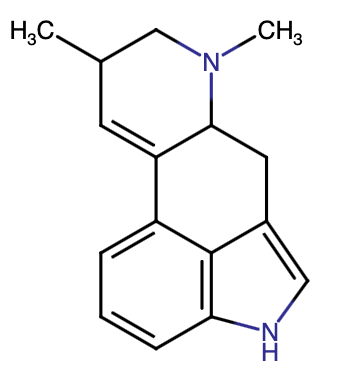
\includegraphics[width=5cm]{lsd-sub.png}

Can you find the price for the compound(s) you found? Do you know the compound with the highest similarity?

\end{document}
%%% Local Variables:
%%% mode: latex
%%% TeX-master: t
%%% End:
